\documentclass[11pt,a4paper]{article}

% ── Packages ──────────────────────────────────────────────────────────────────
\usepackage[utf8]{inputenc}
\usepackage[T1]{fontenc}
\usepackage{lmodern}
\usepackage[margin=2.2cm]{geometry}
\usepackage{graphicx}
\usepackage{booktabs}
\usepackage{multirow}
\usepackage{amsmath,amssymb}
\usepackage{enumitem}
\usepackage{xcolor}
\usepackage{hyperref}
\usepackage{caption}
\usepackage{subcaption}
\usepackage{float}
\usepackage{listings}
\usepackage{titlesec}
\usepackage{fancyhdr}
\usepackage{tcolorbox}

% ── Style ─────────────────────────────────────────────────────────────────────
\hypersetup{colorlinks=true,linkcolor=blue!60!black,citecolor=blue!60!black,urlcolor=blue!60!black}
\definecolor{codebg}{RGB}{245,245,245}
\definecolor{samplebox}{RGB}{235,245,255}

\tcbuselibrary{skins,breakable}
\newtcolorbox{samplebox}[1][]{
  colback=samplebox,colframe=blue!40!black,
  fonttitle=\bfseries,title={#1},
  breakable,boxrule=0.4pt,arc=2pt,left=6pt,right=6pt,top=4pt,bottom=4pt
}

\lstset{
  basicstyle=\small\ttfamily,
  backgroundcolor=\color{codebg},
  breaklines=true,
  frame=single,
  rulecolor=\color{gray!40},
  aboveskip=6pt,belowskip=6pt,
  xleftmargin=4pt,xrightmargin=4pt
}

\pagestyle{fancy}
\fancyhf{}
\fancyhead[L]{\small SLM: Staged Expansion of Small Language Models}
\fancyhead[R]{\small\thepage}
\renewcommand{\headrulewidth}{0.4pt}

\titlespacing*{\section}{0pt}{14pt}{6pt}
\titlespacing*{\subsection}{0pt}{10pt}{4pt}
\setlength{\parskip}{4pt}
\setlength{\parindent}{0pt}

% ── Title ─────────────────────────────────────────────────────────────────────
\title{
  \vspace{-1cm}
  \textbf{SLM: Staged Curriculum Expansion of Small Language Models}\\[4pt]
  \large From 46M to 100M Parameters via Function-Preserving Growth\\
  and Anti-Forgetting Curriculum Training
}
\author{Suyash Bhiste}
\date{April 2026}

\begin{document}
\maketitle

% ── Abstract ──────────────────────────────────────────────────────────────────
\begin{abstract}
We present a staged expansion framework for growing a decoder-only Transformer
language model from 46M to 100M parameters across six training stages.  Starting
from a curriculum-trained TinyStories baseline, the model is progressively
expanded in depth (6$\to$9$\to$12 layers), FFN width (2048$\to$3584), and
context length (256$\to$384$\to$512$\to$768) while being trained on
increasingly complex narrative domains: ROCStories, SimpleStories,
Children-Stories, SimpleWiki, and WritingPrompts.  Each architectural expansion
uses function-preserving or warm-start initialization to minimize output drift.
Catastrophic forgetting is mitigated through TinyStories replay buffers,
Synaptic Intelligence regularization, progressive layer thawing, and
EMA-based forgetting monitoring.  The final 100M-parameter model achieves a
TinyStories perplexity of 5.3 (vs.\ 4.7 at baseline) while reducing
WritingPrompts perplexity from 635 to 42, demonstrating successful
cross-domain generalization with minimal source-domain degradation.
\end{abstract}

\tableofcontents
\newpage

% ── Sections ──────────────────────────────────────────────────────────────────
\section{Introduction}

Training large language models from scratch requires enormous compute budgets.
An alternative strategy is \emph{staged expansion}: begin with a small,
well-trained model and systematically grow its capacity while introducing
progressively harder data.  This report documents such a pipeline, growing a
decoder-only Transformer from 46M parameters (6 layers, $d_\text{ff}=2048$,
context 256) to 100M parameters (12 layers, $d_\text{ff}=3584$, context 768)
across six stages.

\textbf{Key design principles:}
\begin{enumerate}[nosep]
  \item \textbf{Curriculum-driven data.}  Each stage introduces a new domain
        at a controlled mixing ratio, moving from simple children's stories to
        adult fiction.
  \item \textbf{Function-preserving expansion.}  Architectural changes
        (depth, width, context) use initialization strategies that minimize
        initial output drift from the source model.
  \item \textbf{Anti-forgetting suite.}  Replay buffers, Synaptic Intelligence
        regularization, and progressive layer thawing prevent catastrophic
        forgetting of earlier domains.
\end{enumerate}

The six-stage roadmap is:
\begin{center}
\small
\begin{tabular}{clll}
\toprule
\textbf{Stage} & \textbf{Goal} & \textbf{Architecture} & \textbf{New Domain} \\
\midrule
0 & Baseline          & 6L / 2048 / 256 (46M)   & TinyStories \\
2 & Causal chains     & 9L / 2048 / 384 (58M)   & ROCStories + SimpleStories \\
3 & Longer narrative  & 9L / 2048 / 384 (58M)   & Children-Stories \\
4 & Non-fiction style & 12L / 2048 / 512 (71M)  & SimpleWiki \\
5 & Prompt-response   & 12L / 2048 / 512 (71M)  & WritingPrompts (easy) \\
6 & Adult fiction     & 12L / 3584 / 768 (100M) & WritingPrompts (full) \\
\bottomrule
\end{tabular}
\end{center}

\section{Dataset}

The training pipeline draws from seven corpora spanning a difficulty gradient
from age-3 stories to adult fiction.

\begin{table}[H]
\centering\small
\caption{Corpora used across training stages.}
\begin{tabular}{llll}
\toprule
\textbf{Corpus} & \textbf{Source} & \textbf{Character} & \textbf{Val Key} \\
\midrule
TinyStories       & \texttt{roneneldan/TinyStories}         & Simple, ages 3--5      & \texttt{s0}     \\
SimpleStories     & \texttt{SimpleStories/SimpleStories}    & Basic causal stories   & \texttt{simple} \\
ROCStories        & \texttt{mintujupally/ROCStories}        & 5-sentence commonsense & \texttt{roc}    \\
Children-Stories  & \texttt{ajibawa-2023/Children-Stories}   & Longer child narratives& \texttt{child}  \\
SimpleWiki        & \texttt{wikimedia/wikipedia (simple)}   & Encyclopedic, factual  & \texttt{s1}     \\
FineWeb-Edu       & \texttt{HuggingFaceFW/fineweb-edu}      & Educational web text   & \texttt{s2}     \\
WritingPrompts    & \texttt{WritingPrompts (Reddit)}        & Adult fiction, prompts & \texttt{wp}     \\
\bottomrule
\end{tabular}
\label{tab:corpora}
\end{table}

\textbf{Dataset mixing.}
Each expansion stage defines a weighted mixture over corpora.
For example, Stage~2 uses 60\% ROCStories + 40\% SimpleStories, while Stage~6
uses 70\% WritingPrompts + 10\% each of TinyStories, Children-Stories, and
SimpleWiki.  The mixing weights are configured in
\texttt{configs/expansion\_stages.yaml} and implemented via a weighted random
sampling iterator that draws from each corpus proportionally.

\textbf{Train/validation splitting.}
All corpora use a deterministic hash-based split: the MD5 hash of a fixed seed
concatenated with the first 64 characters of each document is computed, and
documents whose hash modulo 10{,}000 falls below a threshold (typically 10\%)
are assigned to the validation set.  This is resume-safe and order-independent,
ensuring the same val set is obtained across runs.  TinyStories uses its
official \texttt{validation} split.

Seven validation sets are maintained and evaluated at every checkpoint across
all stages, enabling consistent cross-domain tracking from Stage~0 through
Stage~6.

\section{Preprocessing}

The preprocessing pipeline converts raw text corpora into fixed-length token
chunks suitable for autoregressive language model training.  It is designed to
support multi-stage curriculum learning with replay buffers and
difficulty-aware sampling.

\subsection{Tokenization and Chunking}

Raw documents are streamed from HuggingFace datasets and processed through a
BPE tokenizer (Section~\ref{sec:tokenizer}).  Each document is wrapped with
\texttt{BOS} (id=2) and \texttt{EOS} (id=3) tokens, producing the sequence:
\[
[\text{BOS}] \;\|\; t_1, t_2, \ldots, t_n \;\|\; [\text{EOS}]
\]
These per-document token sequences are concatenated into a single stream, then
sliced into non-overlapping windows of length $(\texttt{seq\_len} + 1)$.  The
extra token provides the target for the final position (input--target shift).
The last partial window is discarded.

\textbf{Sequence lengths per stage:} Stage~0--3 use $\texttt{seq\_len}=384$,
Stages~4--5 use 512, and Stage~6 uses 768, matching the model's context length
at each expansion.

\subsection{Caching}

All chunked datasets are serialized to disk as \texttt{.pkl} files keyed by
\texttt{(dataset\_name, seq\_len)}.  Subsequent runs load directly from cache,
avoiding re-tokenization.  Mixed-dataset caches use an MD5 hash of the
sorted dataset--weight dictionary as part of the filename to ensure
deterministic cache keys.

\subsection{Difficulty Scoring}

For curriculum-aware modes (\texttt{perplexity}, \texttt{adaptive}), each
story is pre-scored using a composite difficulty metric computed by a
reference model.  Scores are saved in \texttt{curriculum\_scores.npy} as a
$(N, 5)$ array.  Chunk-level difficulties are derived by interpolating story
scores to chunk positions based on their sequential ordering in the dataset.

\subsection{Curriculum Filtering}

In \texttt{adaptive} mode, only a fraction of chunks (sorted by difficulty) is
exposed to the model at any time.  The \texttt{CompetenceScheduler} adjusts
this fraction based on validation improvement rates:
\begin{itemize}[nosep]
  \item Strong improvement ($>$1\% loss decrease) $\to$ expand pool by +5\%
  \item Moderate improvement ($>$0.1\%) $\to$ +2\%
  \item Stagnation for 3 consecutive checks $\to$ forced +1\%
\end{itemize}
The expansion stages use \texttt{random} mode (no curriculum sorting), since
the difficulty gradient is already encoded in the staged domain progression.

\subsection{Anchor Injection}

Regardless of curriculum mode, 10\% of training samples are drawn from an
\emph{anchor pool} consisting of the easiest 5\% of chunks.  This provides
continuous exposure to simple patterns and helps stabilize gradient norms.

\subsection{Replay Pool Preparation}

Each stage loads pre-cached chunks from earlier corpora as a replay buffer.
Source chunks are loaded from the largest available cache file, then:
\begin{itemize}[nosep]
  \item Chunks longer than the target \texttt{seq\_len} are truncated.
  \item Chunks shorter than the target are skipped (not zero-padded, to avoid
        corrupting the loss signal).
\end{itemize}
Replay samples are drawn with probability \texttt{replay\_frac} at each batch
construction, replacing a training chunk with one from the replay pool.

\section{Tokenizer}
\label{sec:tokenizer}

The tokenizer is a Byte-Pair Encoding (BPE) model trained on a combined corpus
using the HuggingFace \texttt{tokenizers} library.  The vocabulary size is
\textbf{50{,}000} sub-word tokens, stored in
\texttt{tokenizers/tokenizer\_corpus.json}.

\textbf{Design choices:}
\begin{itemize}[nosep]
  \item \textbf{BPE over WordPiece or Unigram:}  BPE provides a good balance
        between vocabulary efficiency and handling of out-of-vocabulary tokens.
        It is also the standard for GPT-family models.
  \item \textbf{Corpus-wide training:}  The tokenizer is trained on a combined
        corpus spanning all domains (TinyStories, SimpleWiki, WritingPrompts,
        etc.), ensuring stable tokenization across stages.  A tokenizer trained
        only on children's stories would produce poor segmentation on adult
        fiction vocabulary.
  \item \textbf{Special tokens:}  \texttt{BOS} (id=2) and \texttt{EOS} (id=3)
        delimit documents during chunking.
  \item \textbf{Frozen across stages:}  The same tokenizer is used for all
        six stages.  Changing the tokenizer mid-training would invalidate the
        embedding matrix and cached datasets.
\end{itemize}

\textbf{Vocabulary size trade-off.}  50K tokens is a compromise: large enough
to cover the combined vocabulary with reasonable sub-word granularity, but
small enough that the embedding layer ($50000 \times 512 = 25.6$M parameters
with weight tying) does not dominate the parameter budget.

\section{Positional Encoding}
\label{sec:posenc}

The model supports two positional encoding strategies, configured via the
\texttt{pos\_type} field:

\subsection{Learnable Positional Embeddings (Default)}

The default configuration uses a \textbf{learnable embedding table}
$\mathbf{P} \in \mathbb{R}^{L_\text{ctx} \times d_\text{model}}$, where each
position $i$ has a trainable vector $\mathbf{p}_i$.  The positional signal is
added to the token embedding:
\[
\mathbf{h}_i^{(0)} = \mathbf{E}[x_i] + \mathbf{P}[i]
\]

This approach is simple and effective for fixed-length contexts.  The key
challenge arises during context extension (e.g., 256$\to$384): the new model
has more positions than the trained embedding table.

\textbf{Context extension via interpolation.}
When expanding context length, the positional embedding matrix is extended via
1D linear interpolation along the sequence dimension.  The old embeddings
$(L_\text{old}, d)$ are interpolated to $(L_\text{new}, d)$ using
\texttt{F.interpolate} with \texttt{align\_corners=True}.  Existing positions
retain near-identical values, while new positions receive smooth estimates.
This is applied during Stages~2, 4, and 6.

\subsection{Rotary Position Embeddings (RoPE)}

The model also implements RoPE as an alternative.  RoPE encodes relative
positions directly into the query and key vectors via rotation matrices:
\[
q'_i = \mathbf{R}_{\theta,i} \cdot q_i, \quad k'_j = \mathbf{R}_{\theta,j} \cdot k_j
\]
where $\mathbf{R}_{\theta,i}$ applies rotations at frequencies determined by
$\theta = 10000^{-2k/d}$.  RoPE has the advantage that context extension is
automatic (no learned positions to resize), but the current training uses
learnable embeddings to maintain consistency with the TinyStories baseline.

\section{Base Model Architecture}

The SLM is a decoder-only Transformer with the following design:

\begin{table}[H]
\centering\small
\caption{Base model (Stage~0) architecture.}
\begin{tabular}{ll}
\toprule
\textbf{Component} & \textbf{Specification} \\
\midrule
Vocabulary          & 50{,}000 BPE tokens \\
$d_\text{model}$    & 512 \\
Layers ($n_\text{layers}$) & 6 \\
Heads ($n_\text{heads}$)   & 8 (head dim = 64) \\
FFN width ($d_\text{ff}$)  & 2{,}048 \\
Context length      & 256 \\
Activation          & SwiGLU \\
Normalization       & RMSNorm (pre-norm) \\
Positional encoding & Learnable embeddings \\
Weight tying        & Enabled (tok\_emb = lm\_head) \\
Dropout             & 0.0 \\
Parameters          & 45.8M \\
\bottomrule
\end{tabular}
\end{table}

\textbf{SwiGLU FFN.}
Each layer uses a gated feed-forward network:
$\text{FFN}(x) = W_\text{down} \cdot [\text{SiLU}(W_\text{gate} \cdot x) \odot (W_\text{up} \cdot x)]$,
where $W_\text{gate}, W_\text{up} \in \mathbb{R}^{d_\text{ff} \times d}$ and
$W_\text{down} \in \mathbb{R}^{d \times d_\text{ff}}$.

\textbf{KV Cache.}
For inference, the model implements a key--value cache that pre-fills the prompt
causally and then generates one token at a time.  If the total length exceeds
\texttt{ctx\_len}, it falls back to uncached sliding-window generation.

\textbf{Weight tying.}
The token embedding and LM head share the same weight matrix, reducing the
parameter count by $\sim$25.6M and acting as a regularizer.

\section{Model Architecture Evolution}
\label{sec:expansion}

The model grows through three types of architectural expansion, applied at
specific stages.  Each expansion is validated by measuring cosine similarity
of output logits between the pre- and post-expansion models.

\subsection{Depth Expansion (Layer Cloning)}

\textbf{Applied at:} Stages 2 (6$\to$9 layers) and 4 (9$\to$12 layers).

Selected layers are deep-copied and appended to the model.  Symmetry-breaking
Gaussian noise ($\sigma = 0.01$) is added to all weight matrices (not biases
or norms) in the cloned layers.

\textbf{Why symmetry breaking is mandatory.}
Without noise, cloned layers produce identical gradients and learn identical
functions, providing no capacity benefit.  The noise ensures gradient
differentiation from the first update.

\textbf{Clone selection.}
Layers from the upper half of the network are cloned (e.g., layers [3,4,5] for
6$\to$9).  Upper layers capture more task-specific features, so cloning them
provides useful initialization for learning new domain representations.

\textbf{This is not function-preserving.}
Appending active Transformer blocks changes the model output.  Validation shows
cosine similarity $\approx 0.92$ after depth expansion---indicating significant
but controlled drift.

\subsection{FFN Widening}

\textbf{Applied at:} Stage 6 ($d_\text{ff}$: 2048$\to$3584).

The FFN is widened with function-preserving initialization:
\begin{itemize}[nosep]
  \item $W_\text{gate}$ and $W_\text{up}$: old rows copied, new rows initialized
        with small random values ($\sigma = 0.02/\sqrt{2 \cdot n_\text{layers}}$).
  \item $W_\text{down}$: old columns copied, new columns set to \textbf{zero}.
\end{itemize}
The zero-initialized $W_\text{down}$ columns ensure the new neurons are
\emph{dormant} at initialization---they contribute nothing to the output.
This makes the expansion \textbf{exactly function-preserving}:
$f(x; \theta_\text{expanded}) = f(x; \theta_\text{original})$ for all $x$.

\subsection{Context Length Extension}

\textbf{Applied at:} Stages 2 (256$\to$384), 4 (384$\to$512), and 6
(512$\to$768).

For learnable positional embeddings, the embedding matrix
$\mathbf{P} \in \mathbb{R}^{L_\text{old} \times d}$ is extended to
$\mathbf{P}' \in \mathbb{R}^{L_\text{new} \times d}$ via 1D linear
interpolation (see Section~\ref{sec:posenc}).  This is approximately
function-preserving for positions within the original range.

\subsection{Why Changes Are Staged}

All three expansion types could be applied simultaneously, but staging them
provides several benefits:
\begin{enumerate}[nosep]
  \item \textbf{Controlled drift.}  Each expansion introduces a bounded amount
        of output perturbation.  The training loop can recover from one change
        before the next is applied.
  \item \textbf{Diagnostic clarity.}  If training diverges or forgetting spikes,
        the cause can be attributed to the specific expansion.
  \item \textbf{Curriculum alignment.}  Each expansion is paired with a new
        domain that benefits from the added capacity (e.g., longer context for
        longer stories, wider FFN for richer vocabulary).
\end{enumerate}

\begin{table}[H]
\centering\small
\caption{Architecture at each stage.}
\begin{tabular}{clcccc}
\toprule
\textbf{Stage} & \textbf{Expansion} & \textbf{Layers} & $d_\textbf{ff}$ &
\textbf{ctx} & \textbf{Params} \\
\midrule
0 & (baseline)                   & 6  & 2048 & 256 & 45.8M \\
2 & +3 layers, ctx 384           & 9  & 2048 & 384 & 58.4M \\
3 & (data-only)                  & 9  & 2048 & 384 & 58.4M \\
4 & +3 layers, ctx 512           & 12 & 2048 & 512 & 71.1M \\
5 & (data-only)                  & 12 & 2048 & 512 & 71.1M \\
6 & FFN 3584, ctx 768            & 12 & 3584 & 768 & 99.5M \\
\bottomrule
\end{tabular}
\label{tab:stages}
\end{table}

\section{Catastrophic Forgetting Mitigation}

Training on new domains risks degrading performance on earlier ones.  The
pipeline employs four complementary strategies.

\subsection{Replay Buffers}

Each stage loads pre-cached chunks from earlier corpora as a replay pool.  At
each batch construction, with probability \texttt{replay\_frac} a training
chunk is replaced with one sampled uniformly from the replay pool.

\textbf{Configuration:}
\begin{itemize}[nosep]
  \item Initial replay fraction: 15\% of samples.
  \item Replay cap: 35--40\% (stage-dependent).
  \item EMA-based adaptive scaling: if TinyStories forgetting exceeds
        thresholds, \texttt{replay\_frac} is increased by
        $\text{scale} \times \text{forgetting\_ema}$ (scale $= 3.0$).
  \item Replay sources accumulate: Stage~3 replays from TinyStories and
        ROCStories; Stage~6 replays from TinyStories and Children-Stories.
\end{itemize}

\subsection{Anchor Validation Baseline}

Before training begins at each stage, the TinyStories validation loss is
computed and stored as an \emph{anchor value}.  Throughout training,
forgetting is defined as:
\[
\text{forgetting} = \frac{L_\text{ts}^\text{current} - L_\text{ts}^\text{anchor}}
                         {\max(L_\text{ts}^\text{anchor},\; 10^{-6})}
\]
This relative metric is tracked both raw and as an exponential moving average
(EMA, $\alpha = 0.1$), and logged at every evaluation step.

\subsection{Synaptic Intelligence (SI)}

SI maintains per-parameter importance estimates accumulated during training.
A quadratic penalty is added to the loss:
\[
\mathcal{L}_\text{SI} = \lambda_\text{SI} \sum_k \Omega_k (\theta_k - \theta_k^*)^2
\]
where $\Omega_k$ is the importance of parameter $k$ and $\theta_k^*$ is its
value at the end of the previous stage.  $\lambda_\text{SI}$ ranges from
0.015 to 0.02 across stages.  The $\Omega$ matrices are saved alongside
checkpoints (\texttt{si\_omega\_stage\_N.pt}).

\subsection{Progressive Layer Thaw}

During architectural expansions (Stages~4 and 6), the bottom 3 layers are
initially frozen.  If forgetting exceeds a threshold (5\%), layers are
progressively unfrozen from bottom to top.  This ensures that early
representations---which encode fundamental linguistic features---are
preserved during the initial adaptation phase.

\subsection{Measuring Forgetting}

Forgetting is monitored through:
\begin{enumerate}[nosep]
  \item \texttt{ts\_forgetting}: raw relative forgetting vs.\ anchor.
  \item \texttt{ts\_forgetting\_ema}: smoothed EMA of forgetting.
  \item Cross-domain val loss: all 7 val sets are evaluated at every
        checkpoint, regardless of the active training domain.
\end{enumerate}
\vspace{2pt}
The final Stage~6 model achieves TinyStories val loss of 1.669
(anchor: 1.734), corresponding to \textbf{negative forgetting} ($-3.8\%$),
indicating the model actually \emph{improved} on the source domain.

\section{Training Strategy}

\subsection{Optimization}

All stages use AdamW with $\beta = (0.9, 0.95)$ and weight decay 0.1.
Learning rates use cosine decay with linear warmup:

\begin{table}[H]
\centering\small
\caption{Training hyperparameters per stage.}
\begin{tabular}{ccccccc}
\toprule
\textbf{Stage} & \textbf{LR} & \textbf{Warmup} & \textbf{Batch} &
\textbf{Seq} & \textbf{Max Tokens} & \textbf{Patience} \\
\midrule
2 & $1.5 \times 10^{-4}$ & 1000 & 24 & 384 & 300M & 15 \\
3 & $1.5 \times 10^{-4}$ & 1000 & 24 & 384 & 300M & 15 \\
4 & $1.0 \times 10^{-4}$ & 1000 & 16 & 512 & 400M & 15 \\
5 & $1.0 \times 10^{-4}$ & 1000 & 16 & 512 & 500M & 15 \\
6 & $8.0 \times 10^{-5}$ & 1500 &  8 & 768 & 600M & 15 \\
\bottomrule
\end{tabular}
\end{table}

\textbf{Differential learning rates.}
At expansion stages (2, 4, 6), pretrained parameters receive a lower learning
rate (\texttt{pretrained\_lr\_mult} = 0.5) while newly initialized parameters
(cloned layers, widened FFN columns) use the full rate.  This prevents
catastrophic unlearning of pretrained weights during early training.

\subsection{Early Stopping}

Training terminates via a \emph{relative plateau detector}.  The target
validation metric (determined by \texttt{val\_key}) is monitored with patience
of 15 evaluation intervals.  A relative minimum delta of 0.1\% is used, along
with a minimum token count before exit is allowed (20--30M tokens depending on
stage).  All stages in this run exited via \texttt{plateau}.

\subsection{Gradient Clipping}

Global gradient norm is clipped to 1.0.  Both global and deep-layer gradient
norms are logged to detect instability during expansion.

\section{Results and Evaluation}

\subsection{Cross-Domain Validation Loss}

Table~\ref{tab:results} reports final validation loss and perplexity across
all seven domains at the end of each expansion stage.

\begin{table}[H]
\centering\small
\caption{Final validation loss / perplexity per domain and stage.  Bold
indicates the best result for each domain.  The target domain for each stage
is marked with $\star$.}
\label{tab:results}
\begin{tabular}{l|ccccc}
\toprule
\textbf{Domain} & \textbf{S2 (58M)} & \textbf{S3 (58M)} & \textbf{S4 (71M)}
& \textbf{S5 (71M)} & \textbf{S6 (100M)} \\
\midrule
TinyStories (s0)
  & \textbf{1.649} / 5.2  & 1.648 / 5.2  & 1.641 / 5.2
  & 1.697 / 5.5  & 1.667 / 5.3 \\
SimpleWiki (s1)
  & 7.516 / 1837 & 6.139 / 464  & \textbf{4.137}$^\star$ / \textbf{62.6}
  & 4.341 / 76.8 & 4.449 / 85.5 \\
FineWeb-Edu (s2)
  & 7.413 / 1657 & 6.070 / 433  & \textbf{5.210} / \textbf{183}
  & 5.244 / 189  & 5.312 / 203  \\
ROCStories (roc)
  & \textbf{2.711}$^\star$ / \textbf{15.0}
  & 3.259 / 26.0 & 3.577 / 35.8 & 3.609 / 36.9 & 3.630 / 37.7 \\
SimpleStories
  & \textbf{1.839} / \textbf{6.3}
  & 1.853 / 6.4  & 1.910 / 6.8  & 2.547 / 12.8 & 2.558 / 12.9 \\
Children (child)
  & 4.752 / 116  & \textbf{2.814}$^\star$ / \textbf{16.7}
  & 2.583 / 13.2 & 2.919 / 18.5 & 2.984 / 19.7 \\
WritingPrompts (wp)
  & 6.186 / 486  & 5.854 / 349  & 5.393 / 220
  & 3.797$^\star$ / 44.5
  & \textbf{3.743}$^\star$ / \textbf{42.1} \\
\bottomrule
\end{tabular}
\end{table}

\textbf{Key findings:}
\begin{itemize}[nosep]
  \item \textbf{TinyStories retention is excellent.}  Val loss stays between
        1.641 and 1.697 across all stages (baseline: 1.537).  The net
        degradation of ${\sim}0.13$ corresponds to a perplexity increase
        from 4.7 to 5.3---minimal given the model grew from 46M to 100M
        parameters and was trained on 5 new domains.
  \item \textbf{WritingPrompts drops from PPL 635 to 42.}  The staged approach
        successfully bridges the gap from children's stories to adult fiction.
  \item \textbf{SimpleWiki PPL drops from 2879 to 63.}  The introduction of
        encyclopedic text in Stage~4 dramatically improves factual language
        modeling.
  \item \textbf{ROCStories peaks at Stage~2.}  Since ROCStories is the
        target domain in Stage~2 and is gradually diluted in later stages,
        its val loss increases slightly (2.71$\to$3.63)---an expected
        trade-off of training on increasingly complex domains.
\end{itemize}

\subsection{Stage Summary}

\begin{table}[H]
\centering\small
\caption{Training summary per stage.}
\begin{tabular}{cccccl}
\toprule
\textbf{Stage} & \textbf{Steps} & \textbf{Tokens} & \textbf{Time} &
\textbf{Exit} & \textbf{Target Val} \\
\midrule
2 & 15{,}000 & 138M & 69 min & plateau & roc: 2.711 \\
3 & 15{,}000 & 138M & 69 min & plateau & child: 2.814 \\
4 & 15{,}000 & 123M & 77 min & plateau & s1: 4.137 \\
5 & 15{,}000 & 123M & 77 min & plateau & wp: 3.797 \\
6 & 15{,}000 &  92M & 79 min & plateau & wp: 3.743 \\
\bottomrule
\end{tabular}
\end{table}

Total training compute: $\sim$6.4 hours on a single NVIDIA RTX 4060 Ti (16~GB).

\subsection{Learning Curves}

\begin{figure}[H]
\centering
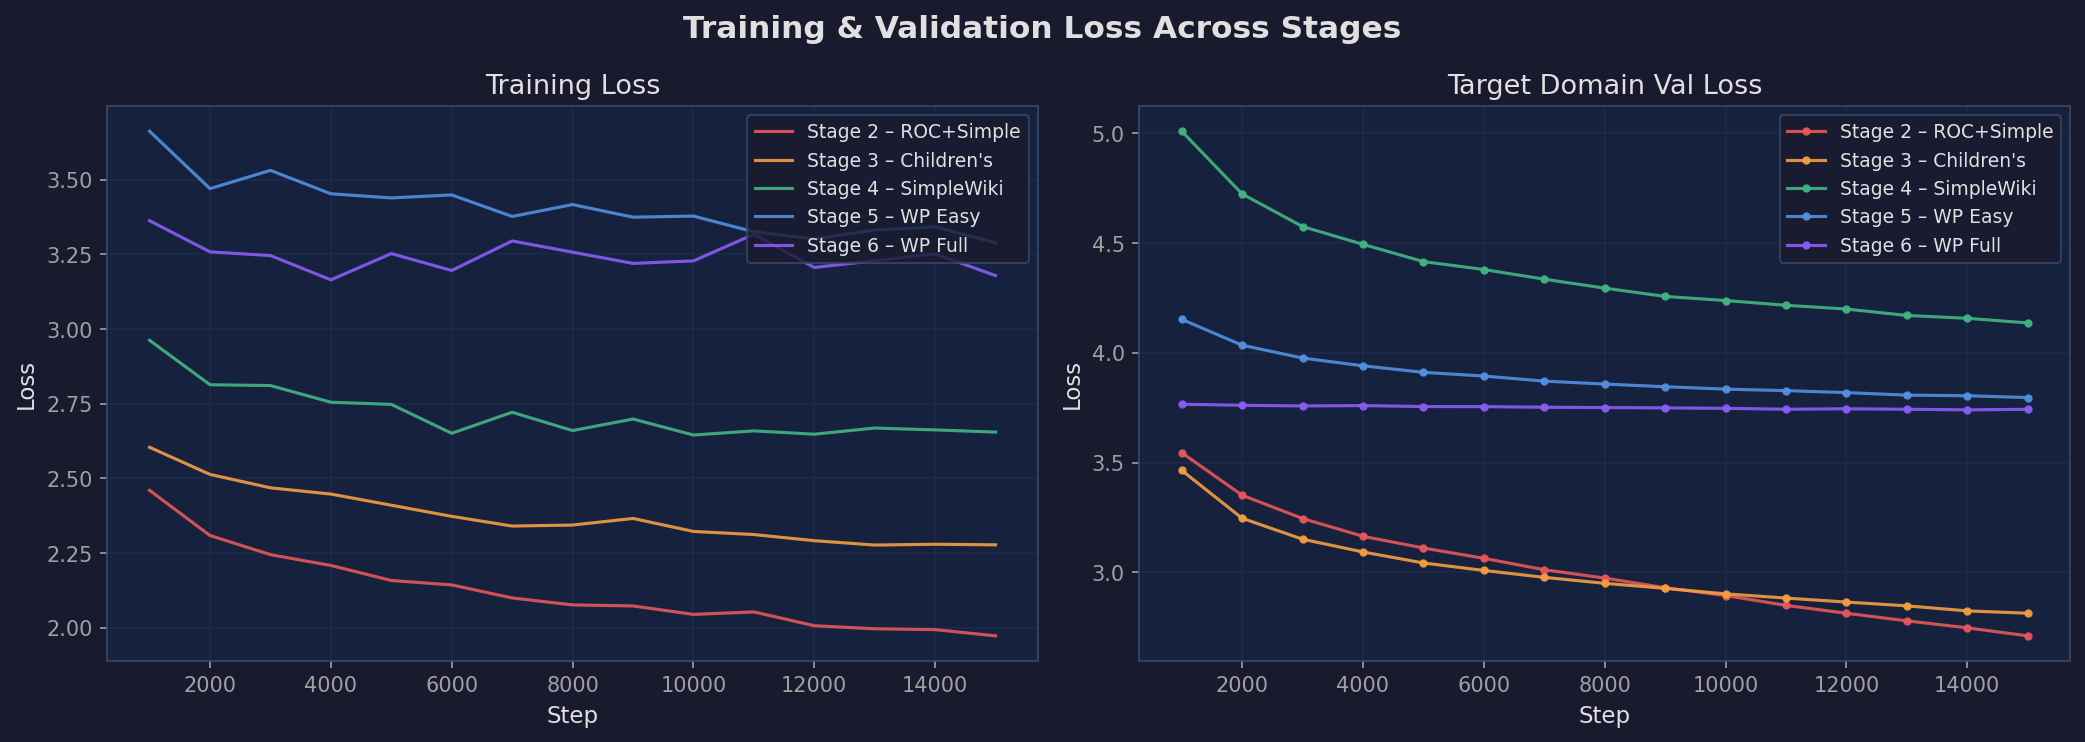
\includegraphics[width=\textwidth]{figures/01_train_val_loss.png}
\caption{Training loss (left) and target domain validation loss (right) across
all five expansion stages.  All stages converge smoothly; later stages have
higher absolute loss due to harder target domains.}
\label{fig:train_val}
\end{figure}

\begin{figure}[H]
\centering
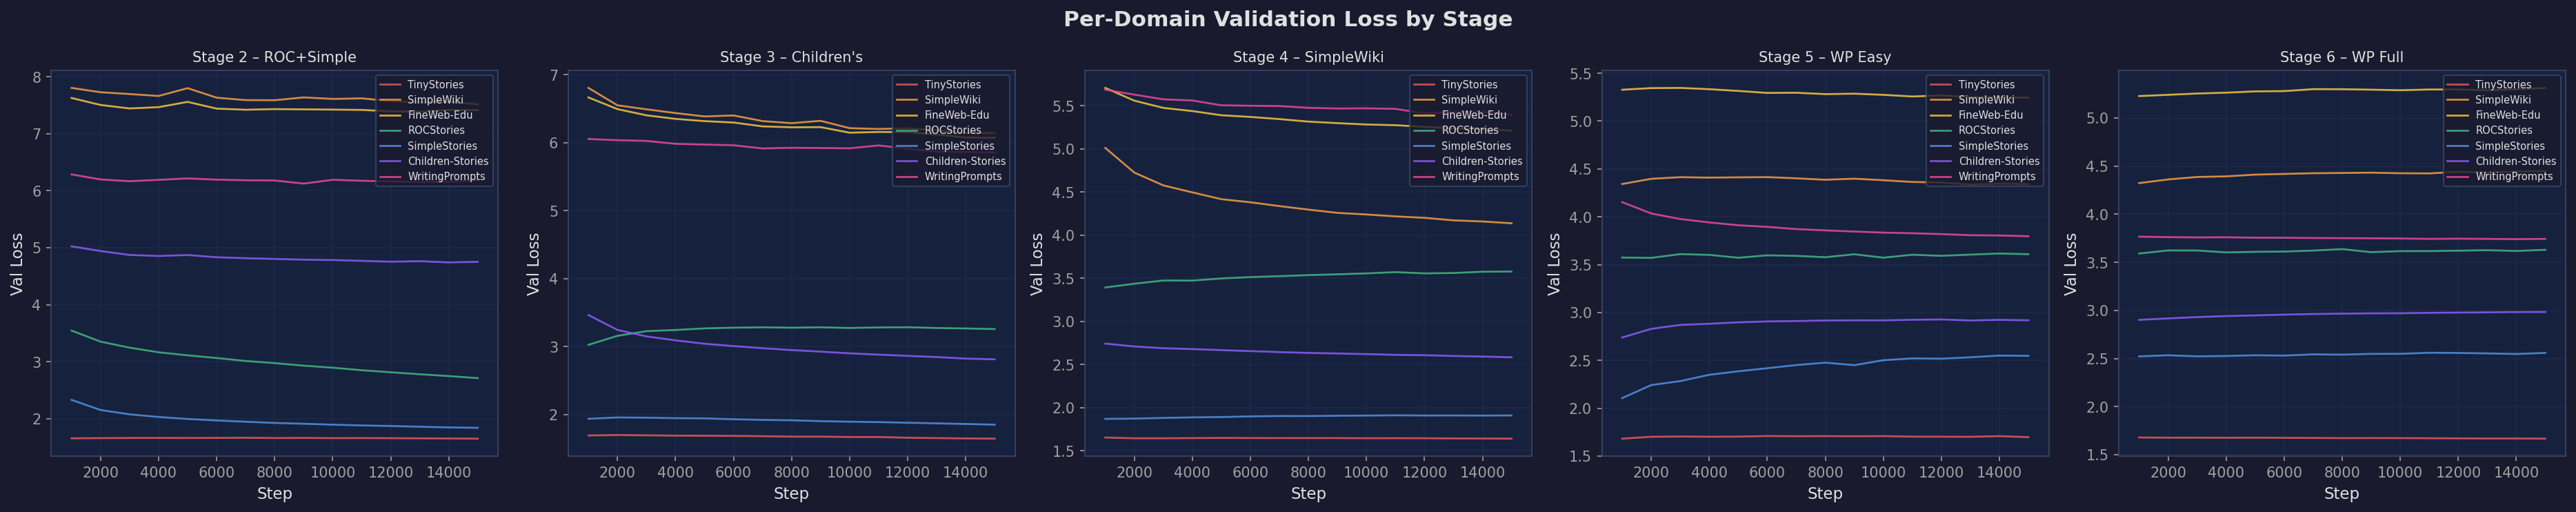
\includegraphics[width=\textwidth]{figures/02_domain_val_loss.png}
\caption{Per-domain validation loss breakdown for each stage.  Note how
TinyStories (red) remains consistently low across all stages, while the
target domain for each stage shows the steepest descent.}
\label{fig:domain_val}
\end{figure}

\begin{figure}[H]
\centering
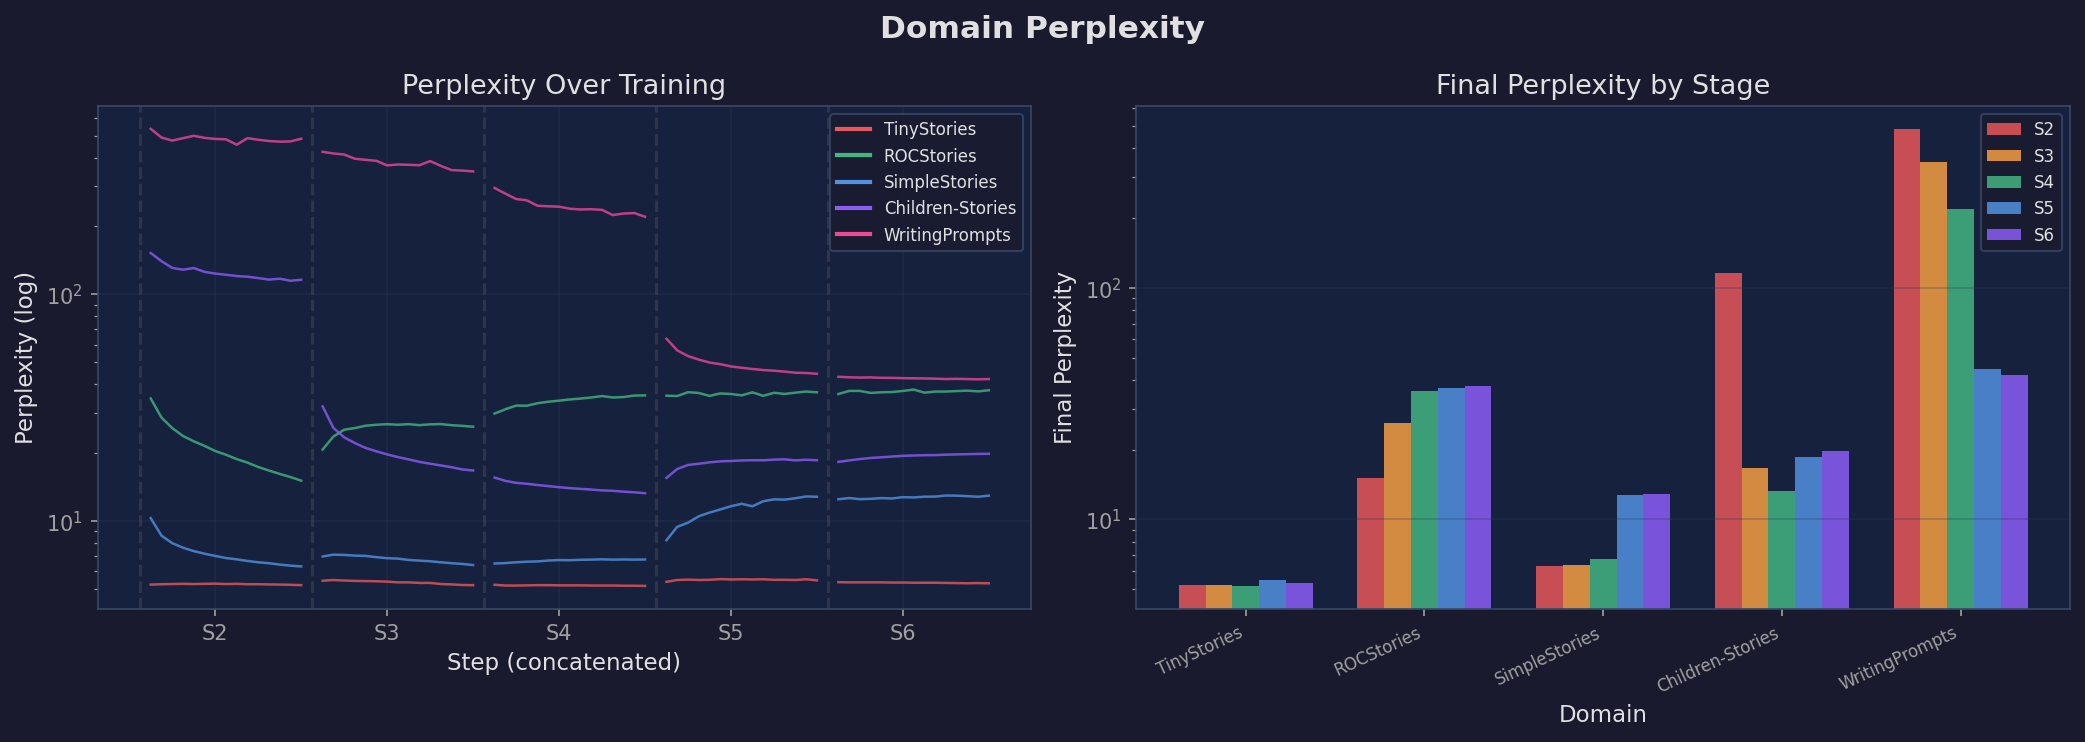
\includegraphics[width=\textwidth]{figures/03_domain_perplexity.png}
\caption{Left: log-scale perplexity over training (stages concatenated).
Right: final perplexity by domain and stage.  WritingPrompts and
Children-Stories show the most dramatic improvements.}
\label{fig:perplexity}
\end{figure}

\begin{figure}[H]
\centering
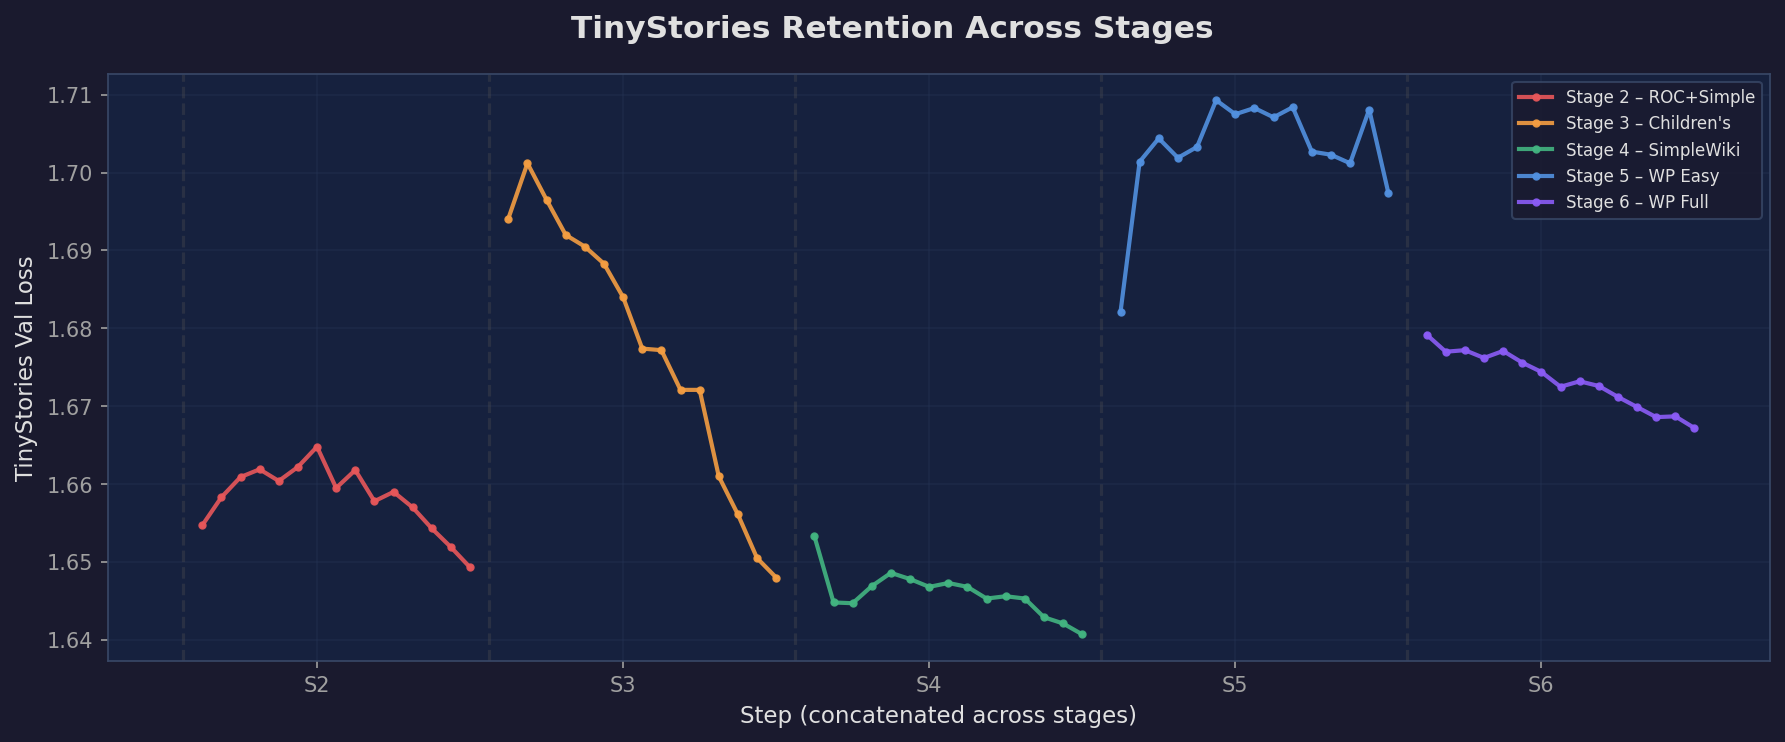
\includegraphics[width=\textwidth]{figures/09_tinystories_retention.png}
\caption{TinyStories validation loss across all stages, demonstrating stable
retention of the source domain.  The total range is only 1.64--1.71.}
\label{fig:retention}
\end{figure}

\begin{figure}[H]
\centering
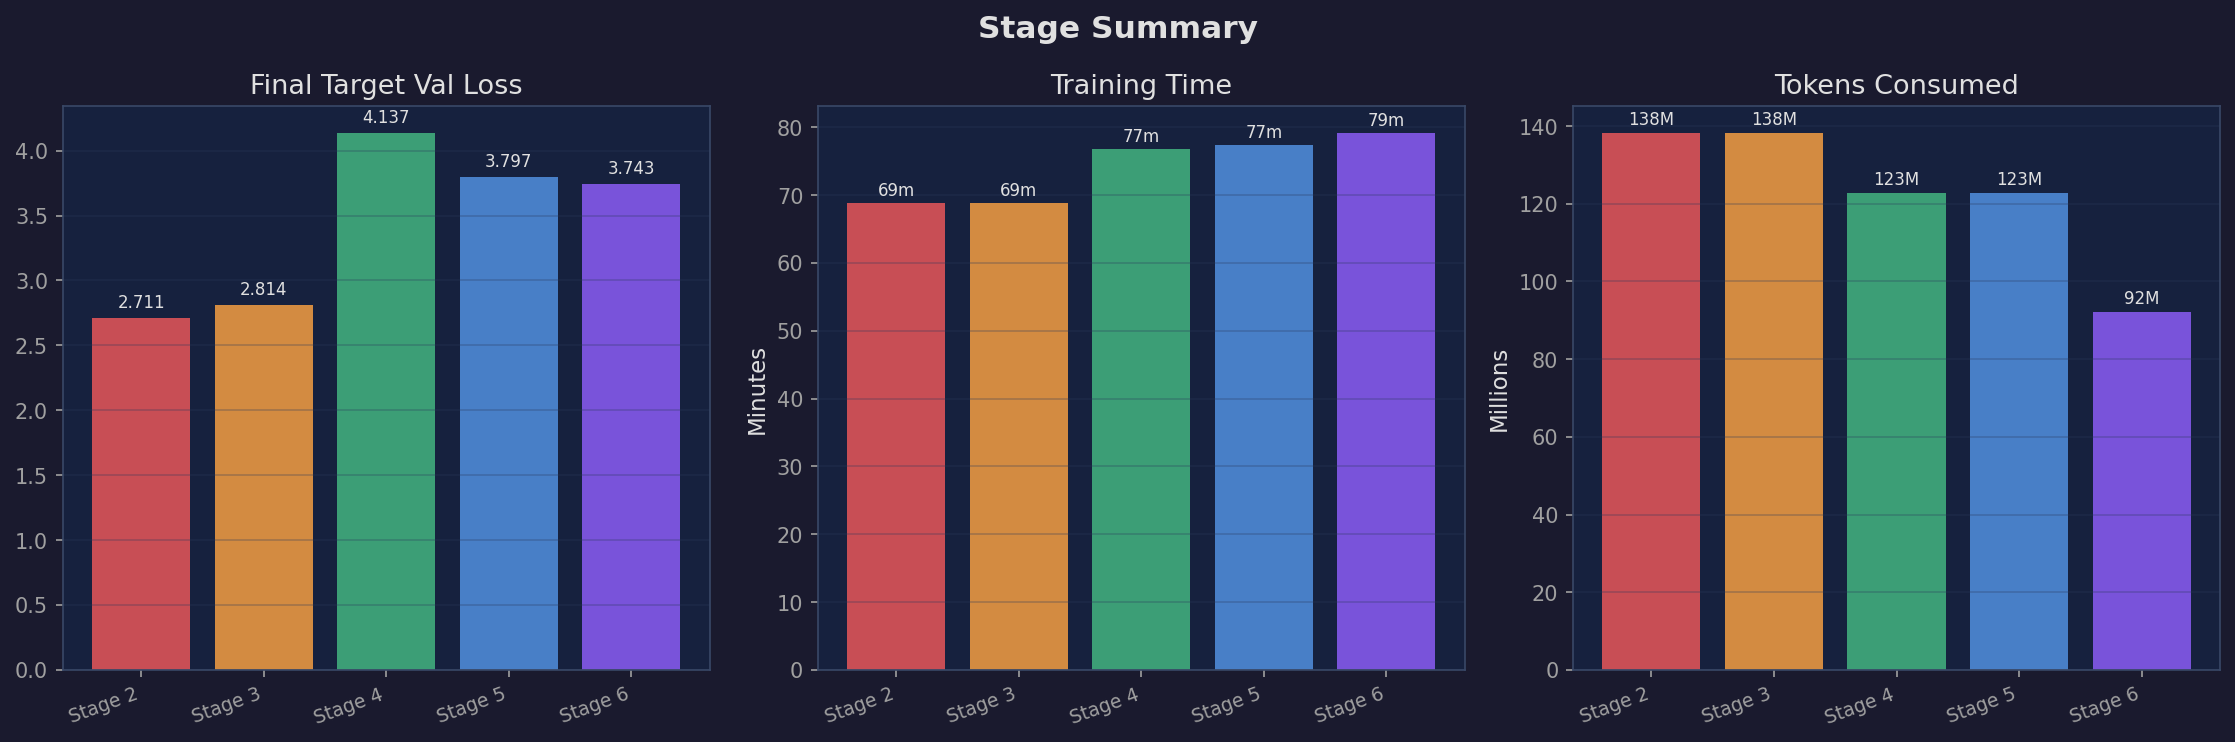
\includegraphics[width=\textwidth]{figures/08_stage_summary.png}
\caption{Stage-level summary: final target val loss, training time, and
tokens consumed.  Later stages process fewer tokens per step due to longer
sequences but take similar wall-clock time.}
\label{fig:summary}
\end{figure}

\begin{figure}[H]
\centering
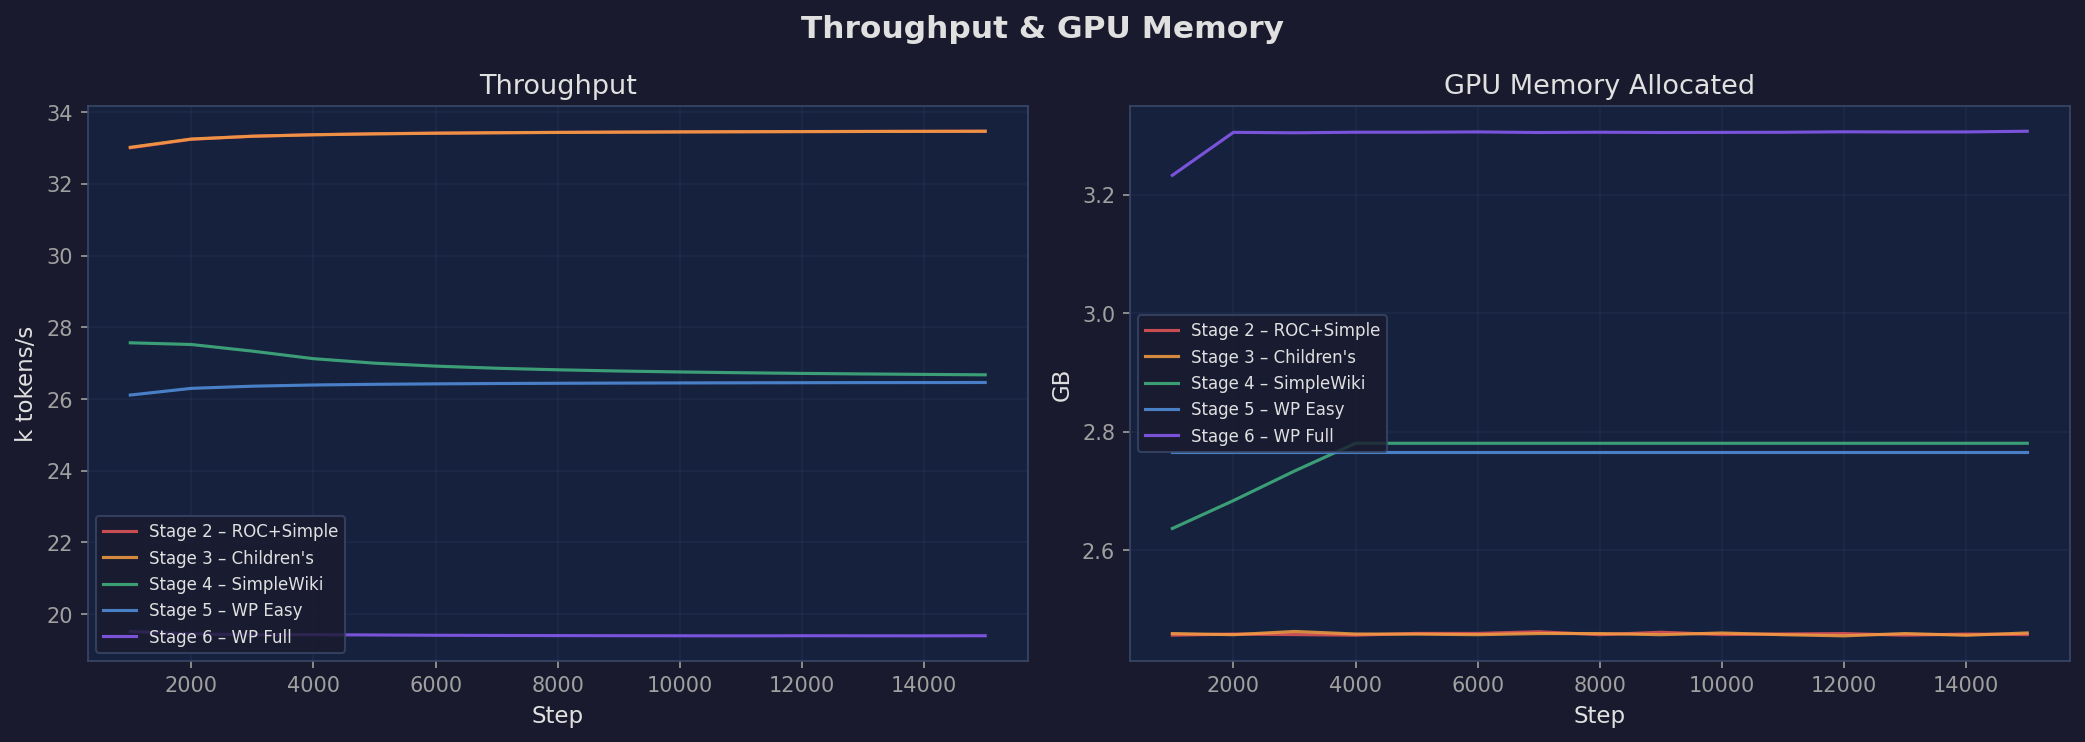
\includegraphics[width=\textwidth]{figures/06_throughput_memory.png}
\caption{Throughput (k tokens/s) and GPU memory allocation across stages.
Stages 4--5 (12 layers, seq 512) and Stage~6 (FFN 3584, seq 768) show
reduced throughput and increased memory usage, as expected.}
\label{fig:throughput}
\end{figure}

\section{Generated Samples}

The following samples are actual outputs from the model at different stages,
generated with temperature 0.7 and top-$k$ = 30.  They demonstrate the
progressive acquisition of stylistic and reasoning capabilities.

\subsection{TinyStories Domain (Ages 3--5)}

\begin{samplebox}[Prompt: ``Once upon a time, there was a little'']
\textbf{Stage 0 (46M):}
Once upon a time, there was a little girl who loved to explore. One day she
went outside and saw a big white cloud in the sky. She thought it was the most
beautiful cloud she had ever seen!

\textbf{Stage 6 (100M):}
Once upon a time, there was a little girl named Lily. She had a pretty dress
that she loved to wear. One day, her mommy said she could go to the store to
buy a new dress. Lily was very excited! At the store, Lily saw a beautiful
dress that she liked\ldots
\end{samplebox}

Both stages produce coherent children's stories.  The Stage~6 model shows
improved entity consistency (Lily is tracked throughout) and more structured
narrative progression, despite being primarily trained on adult fiction in the
later stages.

\subsection{ROCStories Domain (Commonsense Reasoning)}

\begin{samplebox}[Prompt: ``Sarah was excited for her birthday party.'']
\textbf{Stage 2 (58M):}
Sarah was excited for her birthday party. After they were ready, it was time
to see who would win. They both looked at each other and both smiled.

\textbf{Stage 5 (71M):}
Sarah was excited for her birthday party. She ran to the party and said,
``I'm so glad you are here, Sarah!'' But just as Sarah was about to enter the
party, Sarah saw something strange. There was a big fire in the middle of the
park. Everyone was scared\ldots
\end{samplebox}

Stage~5 shows longer, multi-event narratives with scene transitions and
dialogue---capabilities gained through exposure to WritingPrompts.

\subsection{WritingPrompts Domain (Adult Fiction)}

\begin{samplebox}[Prompt: ``The year is 2157. Humanity has'']
\textbf{Stage 0 (46M):}
The year is 2157. Humanity has a lot of time and time. You have to eat more
food and less. You have to be healthy and strong.

\textbf{Stage 5 (71M):}
The year is 2157. Humanity has been in this system for a long time, since the
last humans have been there, and so they have been in their own universe.
They have been in the wrong system for a long time\ldots
\end{samplebox}

\begin{samplebox}[Prompt: ``Death appeared before him and said'']
\textbf{Stage 0 (46M):}
Death appeared before him and said he was not in the end, he was just on the
way in time. The bird was scared and flew away.

\textbf{Stage 6 (100M):}
Death appeared before him and said, ``Dear child, I am Death, and I have come
for you.'' The child was startled and asked, ``But where am I then, Death?''
``You are in the afterlife,'' Death said. ``You will find yourself. You have
been there for a very long time\ldots''
\end{samplebox}

The progression is stark.  Stage~0 cannot handle sci-fi or abstract prompts,
reverting to children's story patterns.  By Stage~6, the model produces
dialogue, maintains a consistent narrative persona (Death as a character),
and sustains multi-turn exchanges---though coherence degrades beyond
$\sim$100 tokens.

\subsection{Cross-Domain Analysis}

\begin{table}[H]
\centering\small
\caption{Qualitative progression summary.}
\begin{tabular}{lp{4cm}p{4cm}p{4cm}}
\toprule
\textbf{Aspect} & \textbf{Stage 0} & \textbf{Stage 3} & \textbf{Stage 6} \\
\midrule
Entity tracking    & Weak (characters change) & Moderate & Consistent across scenes \\
Dialogue           & None                      & Basic quotes & Multi-turn exchanges \\
Narrative length   & 2--3 sentences            & 5--8 sentences & 10+ sentences \\
Domain vocabulary  & Children's only           & Mixed & Sci-fi, drama, abstract \\
Factual content    & N/A                       & N/A & Some Wikipedia-like phrases \\
\bottomrule
\end{tabular}
\end{table}

\input{sections/conclusion}

\end{document}
